\section{Autonomy, capacity and the billion-plus hurdle}
The implemented compiler performs ordinary in-grammar construction without another model call. Validation, replay and acceptance checks are executable. The demonstration and fresh cases were processed automatically once their contracts existed. This is meaningful technical automation, but it does not establish an unattended enterprise: prospect qualification, semantic agreement, buyer authority, exceptions and support remain commercially consequential work.

The model assigns approximately 1.19 human intervention events and 9.17 variable service hours per accepted initial outcome. These are separate quantities: a review intervention can consume hours, and unsuccessful prospects consume effort without creating an accepted outcome. Fixed discovery and research labor is already included in the monetary startup bill. The campaign did not measure a real customer's required human attention, nor infer it from zero human clicks in a synthetic replay.

\subsection{Where the queues bind}
The policy allows eighteen delivery-capacity hours per week and six separately reserved sales/qualification hours. Supported-library orders require three direct construction hours plus an eight-hour aggregate reserve for support, warranty and later obligations. Formation waiting, funding refusal, correction and a contract-level deadline remain visible. The reserve is deliberately conservative, but it does not model a detailed multi-person calendar or prove response-time guarantees during a common incident.

At this reservation rate, one delivery resource has a theoretical ceiling of about 42 orders over 180 days, or 85 per year, before failure, acquisition and renewal constraints. High demand increases accepted orders only from about 7.94 to 11.99 in the tested scenario and increases the expected loss. More agents do not remove buyer acquisition, specialist review, contractual trust or capital obligations. Scaling requires an evidenced change in those constraints.

\subsection{A large industry is not a qualified market}
Primary industry sources provide useful context but not a measured addressable market for this grammar. SPIE's February 2026 issuer release reports roughly 1,600 Photonics West exhibitors and US\$381 billion in 2024 core-component revenue. Photonics21's 2024 report identifies a much broader US\$16 billion instrumentation/optical-measurement category in 2022. Those organizations, definitions and revenue categories cannot be added, and neither establishes eligible EventWeaver customers.\cite{spie,photonics21}

An illustrative funnel of 1,600 directory firms, 10\% eligible, 25\% adopting and two orders per year produces 80 orders and US\$96,000 gross annual revenue. Every funnel fraction is an assumption. At the frozen fee, US\$1 billion in annual revenue would require 833,334 accepted packs. The current narrow offering does not support that volume or its acquisition and service requirements.

The explicit long-horizon ambition is instead \textbf{US\$1 billion of annual net incremental productive value in 2031, measured in constant 2026 dollars relative to the strongest feasible alternative}. A possible arithmetic decomposition is
\begin{equation}
10{,}000\ \text{deployed instruments}\times
\mathrm{US}\$100{,}000\ \text{net annual benefit per instrument}
=\mathrm{US}\$1\ \text{billion/year}.
\end{equation}
Neither adoption nor attributable benefit has been evidenced. Revenue, profit, productive value and valuation are distinct; no valuation is derived from this identity. A route through OEM distribution or a new instrument family would need demonstrated integration, reachable deployments, measured productivity and benefit-sharing terms. The present campaign does not earn a defensible billion-plus thesis.

\section{The successor received a new starting point}
\subsection{A fresh mission that changes the grammar}
The original compiler accepts raw event channel numbers. Its successor adds named virtual references, such as \texttt{stage:heralded\_probe}, allowing an accepted instrument decision to serve as a later instrument's event. The new mission is a heralded detection followed by a conditionally activated calibration-trigger event sequence on other channels. Only Boolean event logic is implemented; no physical calibration is performed. This is a compositional extension, not merely a different lag value or more copies of a supported predicate.

The network must be acyclic, names must resolve, and each consumer observes the previous tick's producer output. All stages read that previous-output snapshot and then update simultaneously. Reset clears the entire network. The original compiler's rejection of virtual references is explicitly tested, establishing that the new wrapper supplies a capability outside its accepted input grammar.

\begin{figure}[htbp]
\centering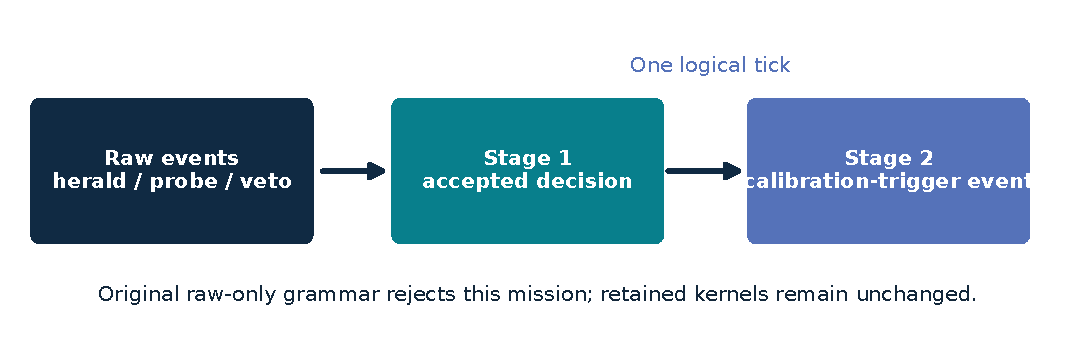
\includegraphics[width=\textwidth]{figures/successor_network.pdf}
\caption{The successor composes unchanged, source-bound kernels through a new acyclic virtual-event interface. One logical tick of interface delay is part of acceptance, not an implementation detail the buyer must guess.}
\end{figure}

The first stage in the demonstration accepts at tick 8; its virtual event reaches the consumer at tick 9; the conditioned stage accepts at tick 14. A later deadline veto cancels a second conditioned decision. Direct RTL wiring between synchronous kernels supplies the previous edge's output; adding another register would incorrectly create a second interface tick.

The demonstration network synthesized to 25 state bits and 65 functional generic cells, plus two Yosys metadata cells. Fresh confirmation used six previously unseen networks and 48 traces, with 10 directed actual-RTL cases covering virtual references in $A$, $B$, $C$ and veto roles, reversed listing order, reset, endpoint veto and a three-stage chain. Twelve bounded equivalence checks passed at depths 16--34.

\subsection{What was inherited, what was rebuilt, what it cost}
The retained asset is the exact predecessor compiler, identified by SHA-256. The wrapper checks that identity. New work includes network grammar validation, virtual-event mapping, graph checks, composition semantics and independent network verification. An ordinary library containing byte-identical compiler and wrapper files was executed in an isolated subprocess and tied. A conventional network wrapping independently authored history kernels also tied functionally.

This result demonstrates productive reuse and a new supported mission. It does not show learned weights, an independently superior specialist or a benefit unavailable from ordinary software reuse. The evidence supports selecting a useful retained artifact, not equating storage with learning.

The extension is charged at US\$3,500 for grammar/integration, validation, fixtures, inference/tools and a failure allowance, plus US\$600 for extraction, validation, integration and first-year storage/upkeep. The total US\$4,100 is included once in the campaign startup account. The conventional identical-library route bears the same retention costs. No commercial surplus funded this extension; it was a separately costed research option within the campaign.

\subsection{The two connected flywheels}
The transformational path has executed links: frontier investigation led to a construction; the construction produced a verified digital capability; that retained capability supported a new compositional instrument. The commercial path reaches an offering and modeled delivery, but stalls before complete-cost surplus. Its missing link cannot be supplied by calling the successor a valuable asset or assuming future growth.

\begin{figure}[htbp]
\centering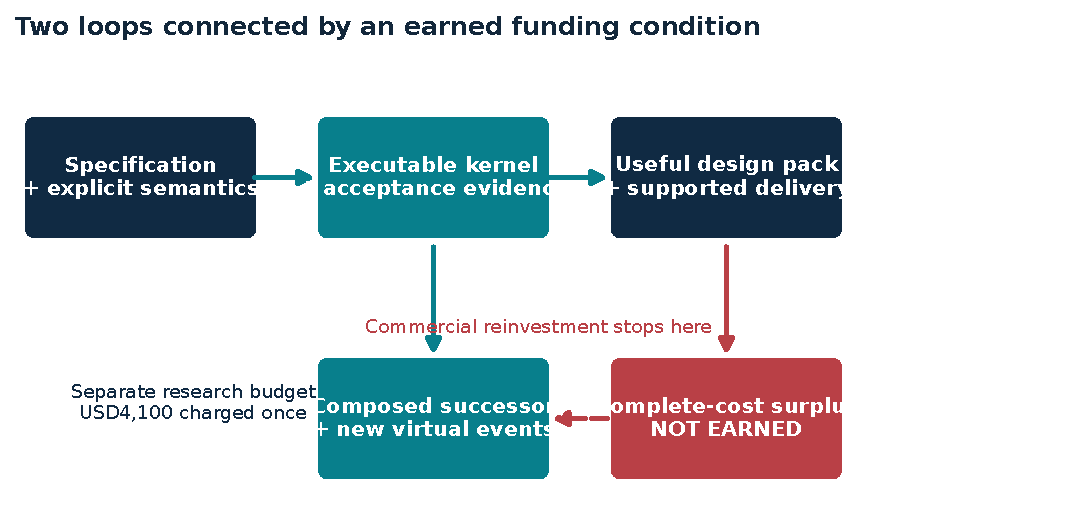
\includegraphics[width=\textwidth]{figures/two_flywheels.pdf}
\caption{The experiment constructs the technical succession link and exposes the unclosed commercial link. A separate research budget is not self-financed compounding.}
\end{figure}

Future surplus would first need to fund buyer-specific interface qualification, timing/throughput evidence, reusable adapters and continued validation. Those means might unlock an integrated measurement offering that this functional kernel cannot yet deliver. The opportunity would support further useful work only if buyers value the integrated outcome above their alternatives and its complete obligations. Neither reinvestment success nor exponential growth is assumed.

\section{Decision: stop this launch and reopen the search}
\textbf{Stop standalone expansion of the frozen US\$1,200 supported-library offering.} The useful construction passes its bounded technical tests, but all tested commercial policies fail to cover full costs and the selected policy loses even before fixed campaign costs. Conventional parity, the negative Python timing result, free-library access and unmeasured demand all constrain the advantage claim.

This is not a proof that every instrumentation enterprise is uneconomic. It is a decision about the selected scope, price, arrangement, acquisition assumptions and obligations. A larger integration problem might justify a different contract and price, but its value cannot be assigned to the small kernel already tested.

\subsection{The failed candidate did not retain the flagship}
After the complete-cost rejection, the campaign returned to the wider possibility search. This was a new, bounded desk investigation recorded on October 28, with priority given to the preceding thirty days and seven days. It did not alter the original selection record, frozen commercial policy or confirmation histories. The stronger question was: what productive capability could change the available actions, and would removing that capability destroy the first valuable outcome?

This \textbf{OUT-TRANSFORM} lens starts with a desired possibility, identifies its binding constraint, invents the means that could remove it, and then asks for a first commercial outcome that actually depends on those means. It does not promote an advisory report or acceptance wrapper when the essential physical or institutional construction is missing. Three serious hypotheses were compared independently of the completed compiler's sunk cost.

\begin{longtable}{L{.21\textwidth}L{.34\textwidth}L{.36\textwidth}}
\caption{Reopened search: consequential possibilities, essential delivery and rejection. The candidates are hypotheses; no second physical or institutional experiment is claimed.}\\
\toprule Possibility & First outcome that requires the construction & Binding gap and campaign decision\\
\midrule\endfirsthead
\toprule Possibility & Essential first outcome & Gap and decision\\\midrule\endhead
Counterfactual experience foundry & A robot recovery controller that succeeds on withheld physical interactions, built from a calibrated generator of scarce training experiences & No robot, physical calibration, model execution, transfer result or paying task. Strongest next investigation, but rejected as this edition's flagship.\\
Local-feedstock material commons & A physically manufactured and tested recipe makes a previously unsuitable local feedstock usable within a declared performance envelope & No samples, assays, accepting producer or complete physical delivery cost. A recipe report would omit the kernel. Reject.\\
Private cross-owner experimental instrument & An authorized joint experiment yields an accepted conclusion that no owner can obtain alone under the same disclosure constraints & No authorized consortium, harmonized measurements or required operation beyond strong free stacks. Synthetic parties would erase the key barrier. Reject.\\
\bottomrule
\end{longtable}

\subsection{The strongest conditional opening: produce informative experience}
The blue-sky possibility is that robots can acquire useful recovery skills from experiences too rare, expensive or destructive to stage repeatedly. The productive object is trustworthy, action-conditioned experience with transferable outcomes. A pile of plausible videos is insufficient. The proposed means is a task-specific world-model/physics hybrid that identifies uncertain physical parameters, generates discriminating recovery interactions, and trains a bounded controller with an explicit validity envelope.

Fresh primary evidence makes this worth investigating. NVIDIA's October 21 Cosmos announcement adds public training tools, simulation checkpoints and Data Factory blueprints. Its repository already includes generation and validation workflows, so those are also incumbent alternatives. Google announced Genie 4 on October 27 as a trusted-tester research preview, with acknowledged physical, spatial and long-session consistency limitations. Gemini Robotics Embodied Reasoning 2 entered public preview the same day, providing high-level reasoning and orchestration that still depends on low-level control interfaces and physical deployment. None of these models was executed in the reopened search.\cite{cosmos,cosmosfactory,genie4,roboticser2}

The first offer would serve one integrator-owned fixture: deliver a recovery controller and calibrated experience generator that achieve an agreed jam/slip recovery on withheld physical instances under fixed time and intervention limits. The buyer is the integrator accountable for throughput. Its strongest alternatives include open Cosmos tooling, competent conventional simulation/domain randomization, demonstration learning and a current-AI-assisted robotics engineer.

The removal test is decisive: hold real data, compute, engineer effort and acceptance fixed, then remove the calibrated counterfactual-generation and parameter-identification loop. An attributed recovery gain should disappear. Replacing a branded tool with a competent substitute must also be tested. If conventional simulation ties at equal or lower complete cost, exclusive kernel advantage fails; a useful integration business would still need independent commercial evidence.

\textbf{No product or paid pilot is claimed.} The campaign had no fixture, physical trace set, calibration or measured buyer benefit. A local analytic or MuJoCo surrogate could test code plumbing, but it would not establish the physical-transfer outcome sold by this offer. Reopening requires actual usable fixture/data access, a named accepting operator, matched baseline and a capped complete-cost experiment. This record does not invent a price, market size or rare-success payoff to manufacture a positive business case.

\subsection{Why the other openings were also rejected}
The local-materials hypothesis would change which heterogeneous feedstocks can be used, through adaptive characterization, recipe generation and batch qualification. The October 20 Saint-Gobain/Microsoft account reports accelerated knowledge construction and hypotheses worth testing; it does not establish our proposed recipe, qualification result or economics. A fair next experiment would make held-out batches from independent feedstock lots and compare conventional experimental design on the same assays, charging failures, disposal and retesting. No such physical construction occurred here.\cite{saintgobain}

The cross-owner hypothesis would change the available scientific action from isolated analysis to an authorized joint experiment. Its missing means includes disclosure control, compatible measurements, governance and participant incentives. DataSHIELD already supplies mature federated analysis with disclosure checks; SecretFlow supplies established secure-aggregation methods. Microsoft's September 29 Quine announcement is relevant scientific context, but access was initially limited to selected research collaborations and fellows, and its reported biology results include wet-lab validation. It cannot be assumed to be this study's accessible production engine.\cite{datashield,secretflow,quine}

The reopened search therefore ends with \textbf{no flagship earned}. That is a bounded campaign result, not a claim that these enterprises are impossible. It protects the next construction from inheriting unsupported commercial significance merely because a predecessor was expensive to build.


\subsection{A narrower retained option: OEM instrument integration}
A separate route for reusing the retained instrument is a \emph{specific OEM-backed integration} in which a composed event decision enables a documented experiment or control sequence beyond installed functions. Swabian's custom-stream/FPGA routes and open acquisition projects provide concrete integration surfaces to investigate. Their existence also supplies a strong incumbent alternative; it is not a presale. This option does not preserve EventWeaver's former flagship claim or displace the reopened cross-domain search.

Reopening the campaign has three bounded evidence gates:
\begin{enumerate}
\item A public-documentation fit study of 30 named platforms, capped at six analyst hours and an estimated US\$810, must identify an actual missing function, a feasible interface and the responsible acceptance role. Stop if the request is already supplied by a standard feature or a simple free extension.
\item A separately authorized buyer-evidence exercise, capped at an estimated US\$1,620, must establish recent real tasks, observed outside costs, failure consequences and a voluntary willingness to commit to a well-defined trial. Model-generated enthusiasm does not satisfy this gate.
\item A customer-backed integration trial must freeze physical/digital acceptance, source/reuse rights, cash terms, cost ceiling and stopping policy before work. A planning cap is not a purchase authorization. Expand only after accepted delivery, final collection, charged support and independently reconstructed positive full-project economics under competent competition.
\end{enumerate}
These gates are designed to resolve the missing commercial bridge with bounded downside. No invented probability of a civilization-scale payoff is multiplied by a large number to justify expenditure. Because the current default is already no expansion, a gate must produce evidence sufficient to change that decision. No buyer outreach or live trial was initiated in this edition.

\subsection{What a successful next result would have to show}
A next offering must add the capability actually needed for its value: a working adapter, an accepted timing contract or another tested construction. It must cover acquisition, failed attempts, verification and warranties, not merely produce a positive delivery margin. Its capacity model must include expert exceptions and common incidents. Its capital must remain available without spending refundable money. Retained assets should improve fresh work after extraction and upkeep, and ordinary-library reuse must remain a control.

The present edition leaves a useful digital construction and a stricter decision rule. Discovery became a construction. The construction became productive digital capacity. The successor obtained a new starting point. The enterprise did not earn the surplus needed to finance that succession, and the renewed search did not earn a replacement flagship. The next opportunity must satisfy the productive and commercial tests on its own evidence.

\section{Continuing AGI Alpha without rewriting its history}
The study follows the existing sequence AGI Alpha, Transformational Intelligence, Out-Learn, Out-Think, Out-Design, Out-Strategise, Out-Execute, Out-Evolve and SUCCESSOR $\Omega$. Actual editions were read rather than substituted with titles or summaries. Their conventional ties, failed integrations, source conditions and physical limits directly shaped this campaign.\cite{ti,economy,tae,outlearn,outthink,outdesign,outstrategise,outexecute,outevolve}

\textbf{Insight} is represented by the evidence-backed candidate and constraint records. The \textbf{Nova-Seed} record binds beneficiary, sources, construction, acceptance, counterevidence, successor and commercial status. These are inspectable local records, not claims of having run an unavailable autonomous discovery service.

\textbf{FusionPlan} uses actual unchanged modules from the pinned repository: plan, protocol, cryptographic support and its vendored ethers dependency. Three EventWeaver work orders compiled and verified locally, while an altered acceptance statement was refused. The resulting plan root and original Git blob hashes are retained. The required positive bounty field is an inert base-unit field in a local plan specification; it is not a funded bounty or a US-dollar quote.

No deployed \textbf{MARK} coordinator or on-chain execution is claimed. File ownership, separate workstreams, explicit contracts and source freezes provide the coordination needed for this bounded campaign. Hashes solve the real problem of identifying the exact artifact tested; tokenization would add no demonstrated commercial value here.

\subsection{Publication and developer handoff}
The deliverable contains the complete paper and LaTeX, browser reader and interactive demonstration, two-page executive brief, runnable construction, conventional controls, simulator, all scenarios, full journal histories, frozen protocols, audit reports, source/claim maps, preserved failures and a developer handoff. The LinkedIn text remains a draft for approval.

Repository policy routes new executable code and HTML through full-source qualification with the existing publication owner. This study therefore uses an isolated additive draft-review route and preserves the canonical publisher. Immutable source and artifact hashes identify the review package. Canonical Pages and a single research-release companion asset require the owner's existing qualification and publication process; a branch or downloadable HTML file is not represented as that completed release.

The handoff identifies the exact remaining actions and forbids using a passive paper-only shortcut for executable work. Existing papers, live contracts, funding arrangements and deployment credentials are not changed by this research edition.
